\section{Kijowski}\label{sec:kijowski}

In 1974, Jerzy Kijowski pursued an axiomatic approach towards a
time-of-arrival quantum distribution. In his paper \parencite{Kijowski}, he sought to compute
the probability distribution for a particle to intersect an hypersurface
$\mathcal{Q}$ immersed in the $(3+1)$-dimensional space-time.
Classically, the trajectory of a particle is a curve in this $3+1$ space
which intersects the hypersurface at a certain point $(\bar{t^{\vphantom{1em}}}, \bar{x^1}, \bar{x^2}, \bar{x^3})$.
An example of a purely
space-like hypersurface is defined by an equation like
$t=\bar{t}$ (which is, more specifically, an hyperplane).
The point coordinates
at which the particle passes through it
essentially tell \emph{where}
the particle is at time $\bar{t}$,
i.e. the values of $\bar{x^1}$, $\bar{x^2}$, $\bar{x^3}$,
given that $\bar{t}$ is known.
For a quantum particle, the exact coordinates $\bar{x^1}$, $\bar{x^2}$, $\bar{x^3}$
are replaced by a complex wavefunction $\psi_{\bar{t}} \in \mathscr{L}^2(\mathbb{R}^3)$
of the variables $x^1$, $x^2$, $x^3$,
where:
$\psi_{\bar{t}}(x^1, x^2, x^3) = \braket{x^1, x^2, x^3}{\psi_{\bar{t}}}$;
$\bra{x^1, x^2, x^3}$ is an eigenbra of the 3-dimensional position operator $\bra{x^1} \ox \bra{x^2} \ox \bra{x^3}$;
and $\ket{\psi_{\bar{t}}}$ is the state ket at time $\bar{t}$ in the ordinary quantum mechanics sense.

The probability that the particle hits this hyperplane at its point of coordinates $x^1, x^2, x^3$
is given by the square modulus $\abs{\psi_{\bar{t}}(x^1, x^2, x^3)}^2$.
More generally, probability distributions are given by bilinear functionals of the wavefunction.

Kijowski then considers an hypersurface that is spanned by one time-like vector and two independent
space-like vectors (as opposed to the purely space-like hypersurface mentioned above).
The time coordinate of the intersection with the \term{world line}
of a particle tells \emph{when} the particle traverses the surface.
(Again, in the quantum sense, such exact value shall be replaced by a probability distribution).
One obvious example would be the hyperplane $x^3 = \bar{x^3}$.
Or, more simply, $x^3 = 0$, which we will consider from now on.

Given all the above considerations, the first requirement is:
\begin{axiom}\label{ax:kijowski:first}
  The probability distribution for the time-of-arrival of a particle at a given surface
  is given by a continuous positive bilinear functional
  \begin{equation*}
    F[\psi_{t}] \eqbydef T_F[\psi_{t}, \psi_{t}] \, \text{.}
  \end{equation*}
\end{axiom}

The reader can classically and intuitively picture an horizontal plane,
a particle below it traveling upwards, and ask the question
``when does the particle pass through?''. The point of intersection,
besides the coordinate $\bar{x^3}$ which is known, and the other two space-like coordinates $\bar{x^1}$ and $\bar{x^2}$,
will have the time coordinate $\bar{t}$ which is the \term{time of arrival} at the hypersurface.

Consistently with the above, Kijowski initially restricted the study to
particles with positive momentum, which in terms of momentum wavefunction
obviously means ${\phi(p^1, p^2, p^3) = 0} \,\, {\forall \, p^3 < 0}$.

The momentum representation $\phi$ is, in fact, used the most in Kijowski's
paper, to make the theory explicit. The rest of this Section will reflect that.

Other requirements for the probability distribution $F[\phi_t]$ are
\begin{axiom}
  $F[\phi_t] \ge 0 \ \forall t$
\end{axiom}
\begin{axiom}
  If $\norm{\phi_t}_{\scriptscriptstyle{\mathscr{L}^2(\mathbb{R}^3)}} = 1 \ \forall t$, then $\int F[\phi_t] \dd t = 1$
\end{axiom}
\begin{axiom}
  $F[\pi(\phi)] = F[\phi]$.
\end{axiom}
In the last one, $\pi$
is the representation of any Galilei transformation
which preserves $\mathcal{Q}$
e.g. a translation which is parallel to the surface
(the first Kijowski paper considered the nonrelativistic case).

From now on, we will consider, for simplicity, the surface $x^3 = 0$.

For reasons of symmetry, in terms of time-of-arrival at $x^3 = 0$,
one intuitively expects a particle
``traveling upwards from the bottom'' to be equivalent
to a particle
``traveling downwards from the top'',
if both position and momentum have their sign flipped.
For a quantum wavefunction in the position representation,
this means
replacing $\psi(\va{x})$ with $\psi(-\va{x})$.
Or $\phi(\va{p})$ with $\phi^{*}(\va{p})$ in momentum representation:
\begin{axiom}
  $F[\phi^{*}_t] = F[\phi_t]$, $\forall t$.
\end{axiom}

The last requirement is that
\begin{axiom}\label{ax:kijowski:last}
    The \term{dispersion}, defined as
    \begin{equation}\label{eq:kijowski:dispersion}
      \int \dd{t} t^2 F[\phi_t] - \qty(\int \dd{t} t F[\phi_t] )^2 \text{,}
    \end{equation}
    is finite.
\end{axiom}

Given the above axioms, Kijowski proved the following
\begin{theorem}
  $\,$

  \begin{enumerate}
    \item
      A specific functional $F_0$ which minimizes the variance
      \eqref{eq:kijowski:dispersion}
      exists;
    \item
      The average value $\int \dd{t} t F[\phi_t] $ is constant over the class of
      functionals defined by the axioms;
    \item
      $F_0$ has the expression
      \begin{multline}\label{eq:kijowski_bilinear_full}
        F_0[\phi_t] = T_{F_0}[\phi_t, \phi_t] = \\
            \frac{1}{m(2\pi\hbar)^4}
            \int\displaylimits_{p_{3}', p_{3}'' \ge 0} \sqrt{p_{3}' p_{3}''} \phi_t^{*}(p_1, p_2, p_{3}') \phi_t(p_1, p_2, p_{3}'')
            \dd p_1 \dd p_2 \dd p_{3}' \dd p_{3}''
                      \, \text{,}
      \end{multline}
  \end{enumerate}
  where the wavefunction is in the momentum representation.
\end{theorem}

Please note that the bilinear $T_{F_0}[\phi_t, \phi_t]$ in the \eqref{eq:kijowski_bilinear_full}
is a particular case of $T_{F_0}[\phi'_t, \phi''_t]$, where $\phi' = \phi'' \eqbydef \phi$.

For a one-dimensional system (or, equivalently, if the system is translation-invariant along the first two axis),
Eq.~\eqref{eq:kijowski_bilinear_full} can be simplified as
\begin{equation}
  \frac{1}{2 \pi m \hbar} \abs{\int_0^{\infty} \dd p \sqrt{p} e^{-\iu p^{2} t / 2m\hbar} \phi_{0}(p)}^2
  \, \text{,}
\end{equation}
where the free evolution
$\phi_t(p) = e^{-\iu p^{2} t / 2m\hbar}\phi_{0}(p)$
is assumed.

While this distribution is ``well behaved'' i.e. it has similar properties of other distributions
associated to quantum observables described by self-adjoint operator and projective measurement,
the corresponding operator found by Kijowski was not self-adjoint and the corresponding
operator-valued measure was not projective.
It was, more weakly, a \term{Positive Operator Valued Measure} or \term{POVM}.
See, for example, \cite[\s 10.3]{TQM1},
for a summary of POVMs, and Chapter~\ref{ch:decohere}.

% Intermediate calculation for to obtain The Book's formulas from Kijowski paper.
%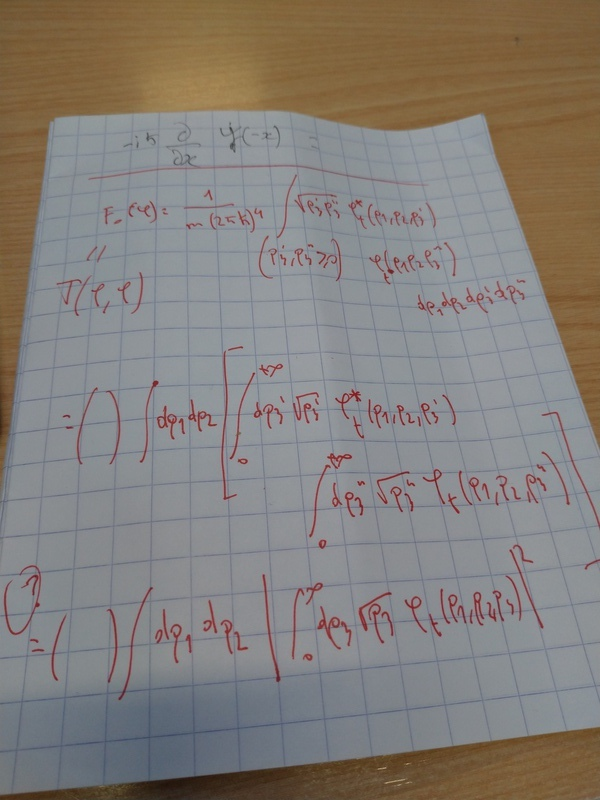
\includegraphics[width=\linewidth]{img/tmp/kijowski1.jpg}
